\subsection{Sele\c{c}\~ao e entrega de conte\'udo}
\paragraph{} Dentro de uma CDN temos que  nos preocupar com a forma como esse conte\'udo vai catalogado, armazenado e distribu\'ido dentro da rede, o que vimos no item \ref{section:protocolos_interacoes}, como tamb\'em temos que nos preocupar como esse conte\'udo vai chegar at\'e o cliente (usu\'ario) da forma mais otimizada poss\'ivel, ou seja, o servidor o qual vai fornecer as informa\c{c}\~oes para ele ser\'a o mais perto ou mais r\'apido. 
\paragraph{} Temos que destacar tamb\'em a import\^ancia da otimiza\c{c}\~ao do fluxo de informa\c{c}\~ao pela rede. Visto que quanto maior o tr\'afico de informa\c{c}\~ao pela rede significa que a informa\c{c}\~ao est\'a mais distante do usu\'ario e tamb\'em que vai ter um custo maior pela troca intensa de informa\c{c}\~ao. 
\paragraph{} Segundo \cite{krishnamurthy2001use}, na tentativa de otimizar o redirecionamentos de URL para o usu\'ario se sacramentou dois tipos de t\'ecnicas de redirecionamentos:
\begin{itemize}
	\item Full - site
	\item Partial - site
\end{itemize}

\subsubsection{Full - site}
\paragraph{} Na t\'ecnica de Full-site todo o conte\'udo \'e entregado ao usu\'ario de um servidor ponta \'unico. Ou seja, o usu\'ario faz uma requisi\c{c}\~ao ao servidor principal, onde o mesmo processa um algoritmo de roteamento para encontrar o servidor ponta que melhor se enquadra como resposta, e ent\~ao retorna ao usu\'ario o endere\c{c}o onde ent\~ao ser\'a consumido por fim todas as informa\c{c}\~oes requisitadas. 
\paragraph{} \'E importante salientar que essa t\'ecnica \'e amplamente utilizada por servi\c{c}os que fazem pouco uso de dados da rede. Uma p\'agina est\'atica da web, por exemplo, se encaixaria perfeitamente nesse contexto. Visto que possui baixo grau de modifica\c{c}\~oes e seu tamanho \'e pequeno perto de outros tipos de m\'idias que circulam na web.

\subsubsection{Partial - site}
\paragraph{} J\'a redirecionamentos do tipo Partial-sites os servideores principais retornam para o usu\'ario uma parte do conte\'udo e disparam, automaticamente, um algoritmo de roteamento para encontrar o restante da informa\c{c}\~ao e retornar ao usu\'ario. Conforme podemos ver na figura \ref{figura:entrega_conteudo}
\begin{figure}[h]
\caption{Entrega de conte\'udo}
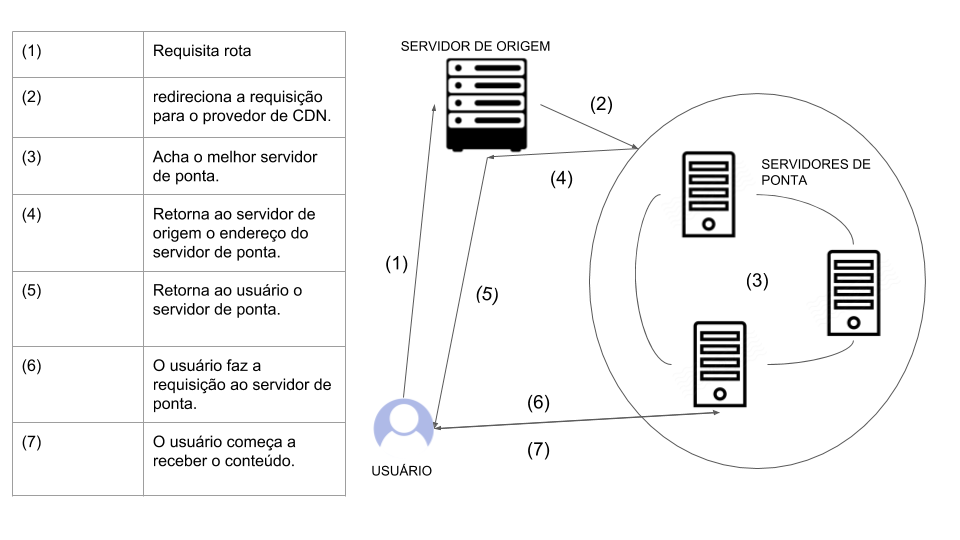
\includegraphics[width=10cm]{Figuras/entrega_conteudo.png} 
\label{figura:entrega_conteudo}
\end{figure}
\paragraph{}  Nela podemos ver que todo o processo acontece em, basicamente, 5 etapas. (1) o usu\'ario faz uma requisi\c{c}\~ao ao servidor principal, depois, em (2) o servidor principal retornar um html com as principais informa\c{c}\~oes e dispara automaticamente (3) um processo de roteamento (4) para buscar o melhor servidor e retornar (5) para o usu\'ario os conte\'udos.
\paragraph{} Entretanto h\'a em (4) diversas formas de fazer esse roteamento quanto a distribui\c{c}\~ao do conte\'udo pela rede e quanto a aglomera\c{c}\~ao desse conte\'udo dentro do servidores de cache. Separamos 2 de cada para explicitar melhor.
\paragraph{} Tipos de distribui\c{c}\~ao:
\begin{itemize}
	\item Empirico
	\item Popularidade
\end{itemize}
\paragraph{} Tipos de aglomera\c{c}\~oes:
\begin{itemize}
	\item Objeto
	\item Conjunto de objetos
\end{itemize}

\subsubsection{Exemplo}

\begin{figure}[h]
\caption{exemplo VOD}
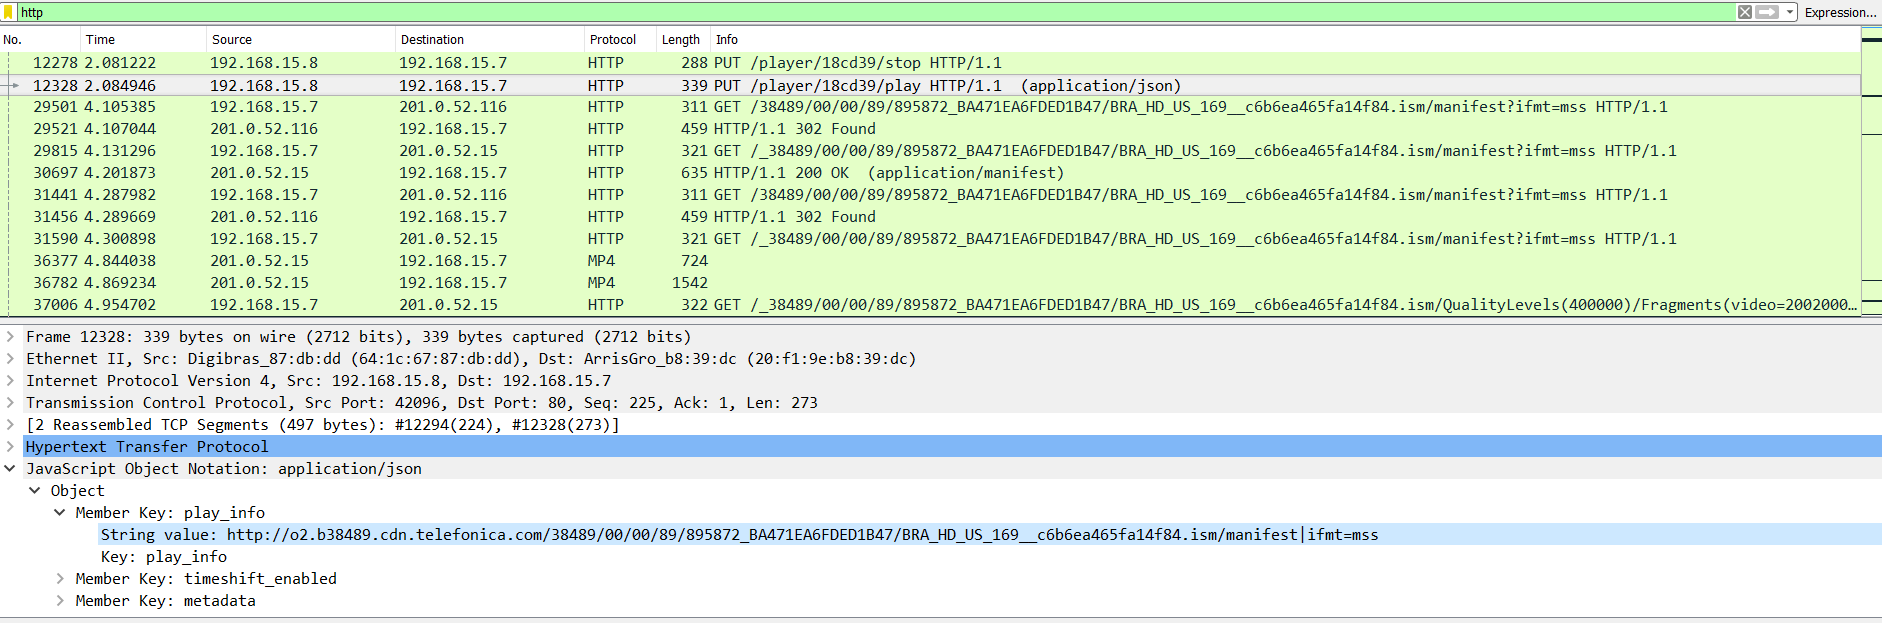
\includegraphics[width=10cm]{Figuras/exemplo_vod_1.png} 
\label{figura:exemplo_vod_1}
\end{figure}

\begin{figure}[h]
\caption{exemplo VOD}
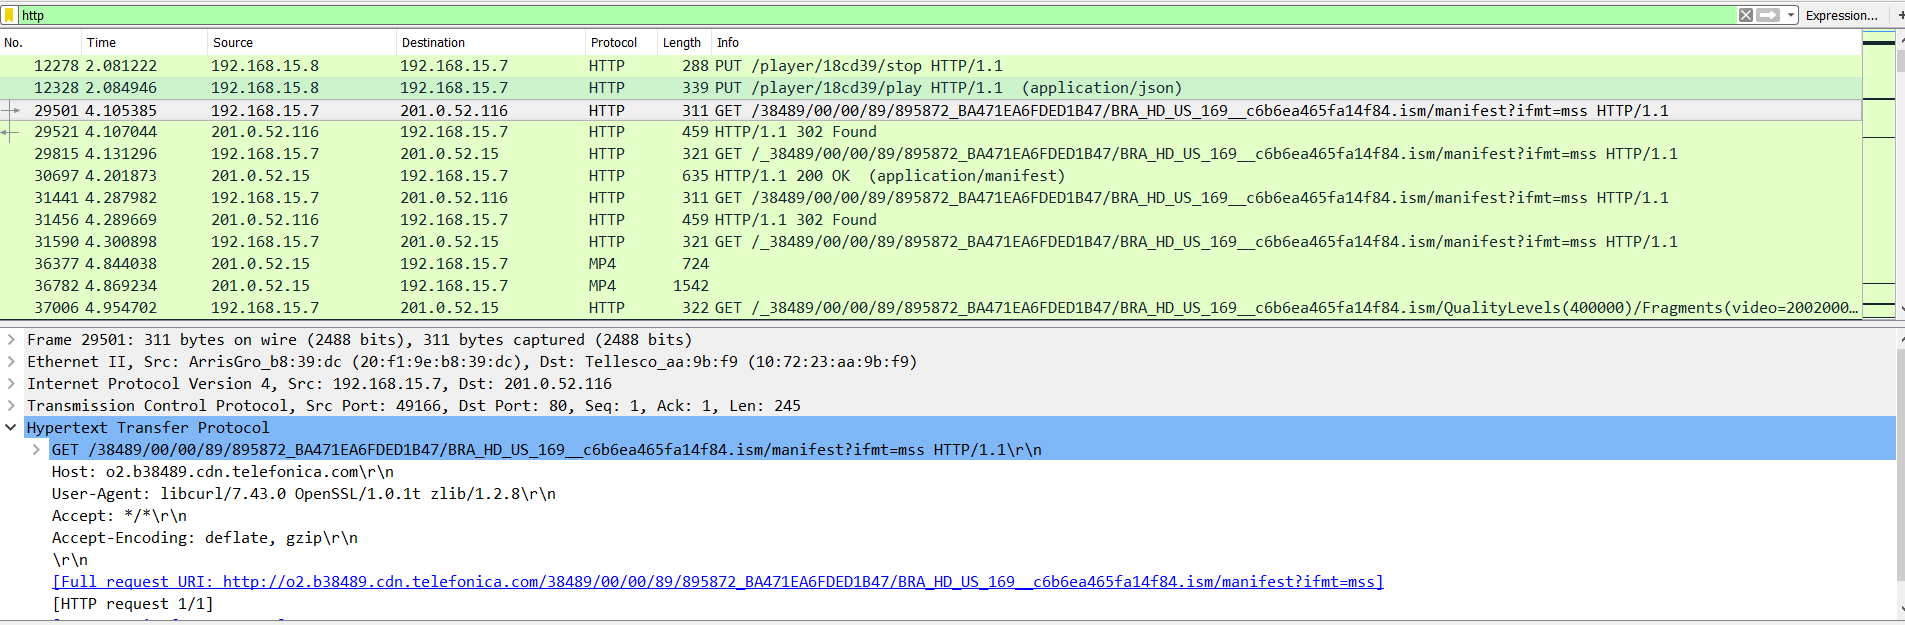
\includegraphics[width=10cm]{Figuras/exemplo_vod_2.png} 
\label{figura:exemplo_vod_2}
\end{figure}

\begin{figure}[h]
\caption{exemplo VOD}
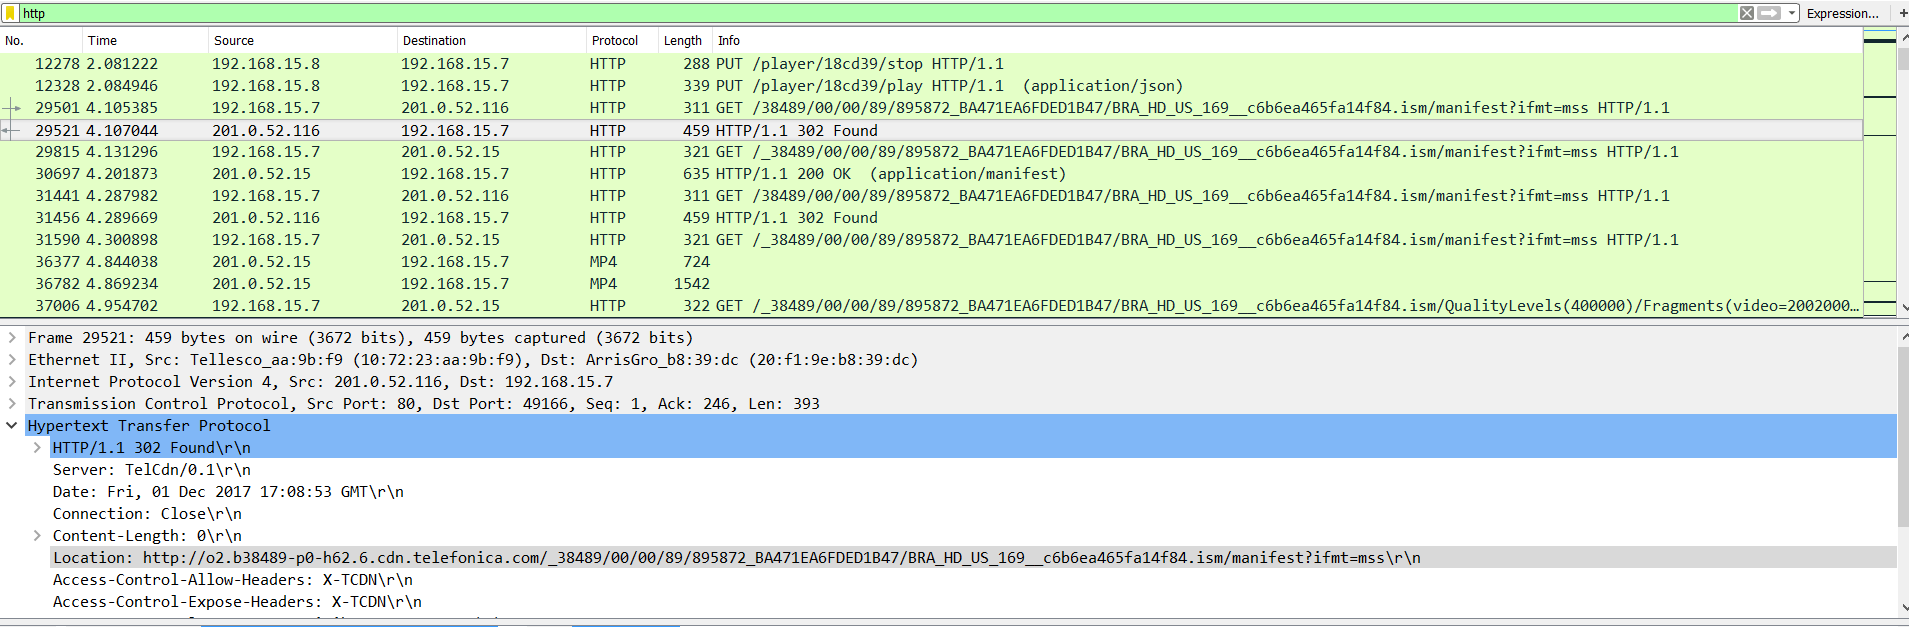
\includegraphics[width=10cm]{Figuras/exemplo_vod_3.png} 
\label{figura:exemplo_vod_3}
\end{figure}

\begin{figure}[h]
\caption{exemplo VOD}
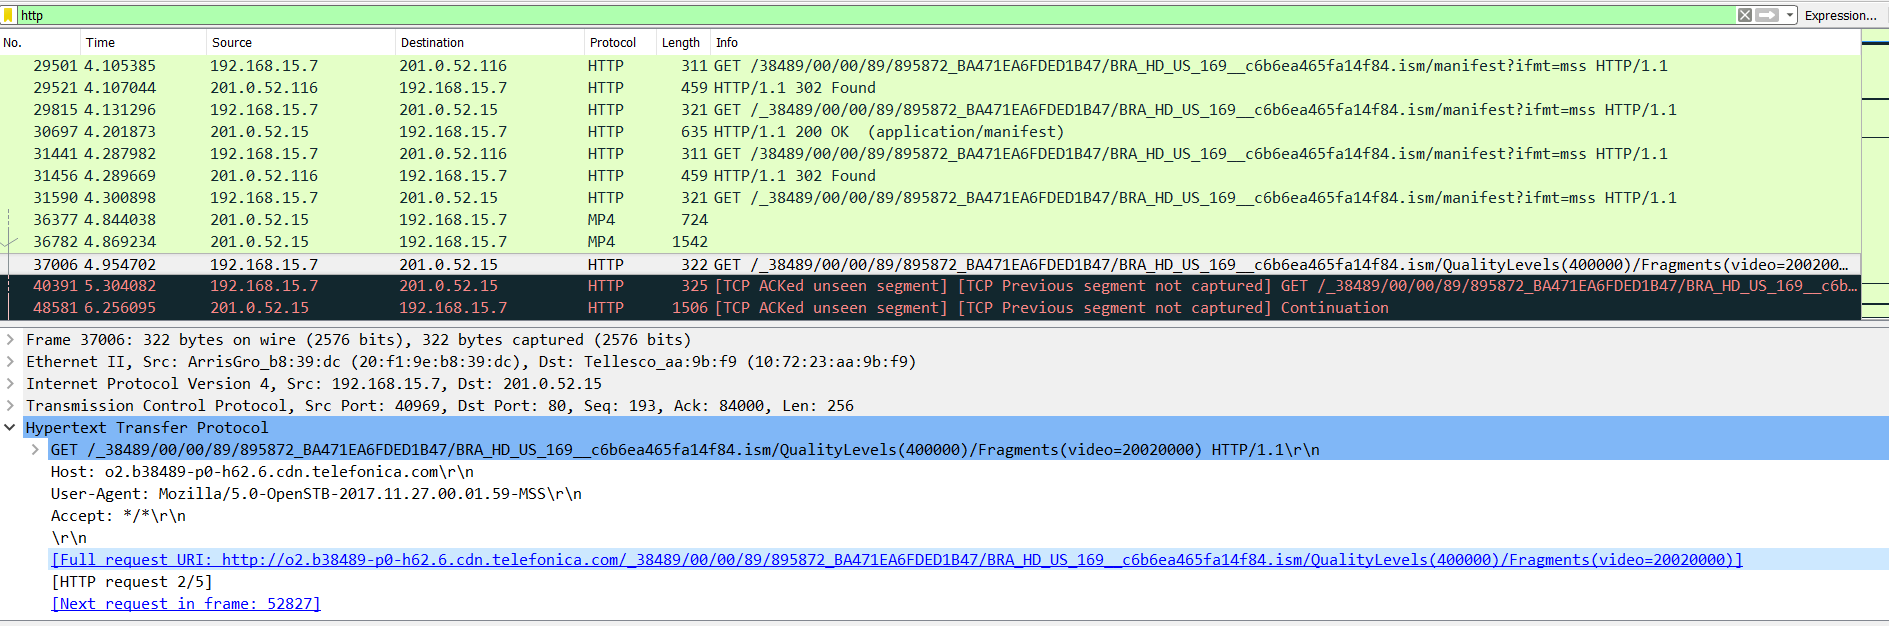
\includegraphics[width=10cm]{Figuras/exemplo_vod_4.png} 
\label{figura:exemplo_vod_4}
\end{figure}